%%%%%%%%%%%%%%%%%%%%%%%%%%%%%%%%%%%%%%%%%
% -- TACTICAL COMPUTING LABORATORIES
% -- LATEX TEMPLATE
%%%%%%%%%%%%%%%%%%%%%%%%%%%%%%%%%%%%%%%%%

%----------------------------------------------------------------------------------------
%	PACKAGES AND DOCUMENT CONFIGURATIONS
%----------------------------------------------------------------------------------------

\documentclass{article}

\usepackage[margin=1.0in]{geometry}
\usepackage[version=3]{mhchem} % Package for chemical equation typesetting
\usepackage{siunitx} % Provides the \SI{}{} and \si{} command for typesetting SI units
\usepackage{graphicx} % Required for the inclusion of images
%\usepackage{natbib} % Required to change bibliography style to APA
\usepackage{amsmath} % Required for some math elements 
\usepackage[utf8]{inputenc}
\usepackage[english]{babel}
\usepackage[parfill]{parskip}
\usepackage{array}
\usepackage{algorithm}
\usepackage{algcompatible}
\usepackage{listings}
\usepackage{xcolor}
\usepackage{courier} % for \texttt{}
\usepackage{dirtree}
\usepackage{pgfgantt}
\usepackage{multirow}
\usepackage{xargs}
\usepackage{xcolor}
\usepackage[colorinlistoftodos,prependcaption,textsize=tiny]{todonotes}
\newcommandx{\unsure}[2][1=]{\todo[linecolor=red,backgroundcolor=red!25,bordercolor=red,#1]{#2}}
\newcommandx{\change}[2][1=]{\todo[linecolor=blue,backgroundcolor=blue!25,bordercolor=blue,#1]{#2}}
\newcommandx{\info}[2][1=]{\todo[linecolor=OliveGreen,backgroundcolor=OliveGreen!25,bordercolor=OliveGreen,#1]{#2}}
\newcommandx{\improvement}[2][1=]{\todo[linecolor=Plum,backgroundcolor=Plum!25,bordercolor=Plum,#1]{#2}}
\newcommandx{\thiswillnotshow}[2][1=]{\todo[disable,#1]{#2}}
\newcommand\mynote[1]{\textcolor{red}{#1}}

\RequirePackage{epstopdf}
\RequirePackage{tabularx}
\RequirePackage{xstring}
\RequirePackage{hyperref}
\RequirePackage{fancyhdr}

%-- setup paragraphs and margins
\setlength{\parindent}{1em}
\setlength{\parskip}{1em}

%-- code listing setup
\lstdefinestyle{base}{
  language=C++,
  numbers=left,
  stepnumber=1,
  emptylines=1,
  breaklines=true,
  basicstyle=\ttfamily\color{black},
  moredelim=**[is][\color{red}]{@}{@},
}

%-- setup hyperlinks
\hypersetup{
  colorlinks=true,
  linktoc=all,
  linkcolor=black,
  citecolor=black,
  urlcolor=black
}
%--

\setlength\parindent{0pt} % Removes all indentation from paragraphs

\renewcommand{\labelenumi}{\alph{enumi}.} % Make numbering in the enumerate environment by letter rather than number (e.g. section 6)

%\usepackage{times} % Uncomment to use the Times New Roman font
%----------------------------------------------------------------------------------------
%	DOCUMENT LAYOUT INFORMATION
%----------------------------------------------------------------------------------------
\pagestyle{fancy}
\lhead{}
\chead{CircusTent}
\rhead{}
\lfoot{Version 1.0} %-- format: TR YYYY-RRR-V.V; y = year; r = report; v = version
\cfoot{CircusTent}
\rfoot{\thepage}      % -- page number

%----------------------------------------------------------------------------------------
%	DOCUMENT INFORMATION
%----------------------------------------------------------------------------------------

\title{CircusTent Developer Guide} % Title

\author{Tactical Computing Laboratories, LLC} % Author name

\date{} % Date for the report

\begin{document}

%-- begin TCL logo
\begin{figure}
\begin{center}

\includegraphics[width=2in]{figures/circus_tent.png} % Include the logo
\end{center}
\end{figure}
%-- end TCL logo

\maketitle % Insert the title, author and date
\thispagestyle{fancy} %-- force the fancyhdr

\begin{center}
\begin{tabular}{l r}
Date: & November 27, 2019 \\ % Date the experiment was performed
Revision: & 1.0 \\         % revision number
Authors: & John D. Leidel\\ % Author names
& jleidel@tactcomplabs.com\\
\end{tabular}
\end{center}

% If you wish to include an abstract, uncomment the lines below
% \begin{abstract}
% Abstract text
% \end{abstract}

%----------------------------------------------------------------------------------------
%       TOC
%----------------------------------------------------------------------------------------

\clearpage
\tableofcontents
\clearpage

%----------------------------------------------------------------------------------------
%       List of Figures
%----------------------------------------------------------------------------------------

\clearpage
\listoffigures
\lstlistoflistings
\listoftables
%\listofalgorithms
\clearpage

%----------------------------------------------------------------------------------------
%	SECTION 1
%----------------------------------------------------------------------------------------
\clearpage
\section{Introduction}
\label{sec:Introduction}

The CircusTent benchmark infrastructure is constructed in a manner that provides
users the ability to extend the existing set of benchmark implementations (herein 
referred to as \textit{Impls}) with additional programming models.  As we see in Figure~\ref{fig:Arch}, 
the CircusTent infrastructure contains a top-level driver object that is manifested as a 
binary executable.  Within this binary executable, we use a set of driver objects that handle 
the initialization and parsing of various runtime options.  We also use a base implementation 
class that is inherited from all other implementations in order to provide a common implementation 
interface.  

\begin{figure}[h]
\begin{center}
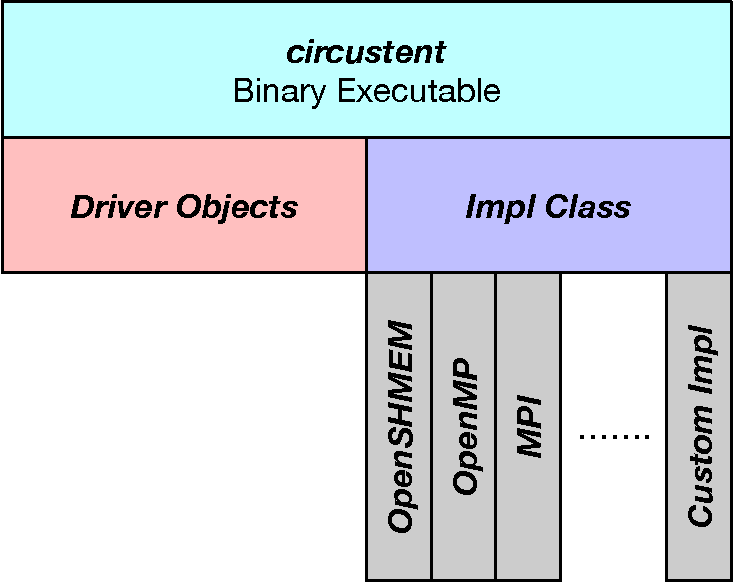
\includegraphics[width=4in]{figures/Arch.pdf}
\vspace*{8pt}
\caption{CircusTent Architecture}
\label{fig:Arch}
\end{center}
\end{figure}

The remainder of this document is organized as follows.  Section~\ref{sec:Building} 
describes the process by which to build CircusTent from source.  Section~\ref{sec:BackendDev} 
describes the process by which to modify the existing portions of the source tree and adding 
the necessary files for new backend implementations.  

%----------------------------------------------------------------------------------------
%	SECTION 2
%----------------------------------------------------------------------------------------
\clearpage
\section{Building CircusTent}
\label{sec:Building}

\subsection{Required Packages}
\label{sec:RequiredPackages}

The following packages are required for developers to build and debug 
new CircusTent backend implementations. 

\begin{itemize}
\item CMake 3.4.3+
\item C/C++ Compiler (GCC and Clang have been tested)
\end{itemize}

Optional packages that may be required include:

\begin{itemize}
\item RPM tools to build platform RPMs
\item Debian package tools (deb) for constructing DEB binary payloads
\item Backend specific libraries, runtimes and tool chains
\item System/platform/API debuggers
\end{itemize}

\subsection{Building From Source}
\label{sec:BuildingFromSource}

Building the CircusTent infrastructure can be performed using the following 
steps.

Clone the CircusTent repository:
\begin{verbatim}
$> git clone https://github.com/tactcomplabs/circustent.git
\end{verbatim}

Setup your build tree:
\begin{verbatim}
$> cd circustent
$> mkdir build
$> cd build
\end{verbatim}

Execute CMake to generate the makefiles (where XXX refers 
to the backend that you wish to enable).
\begin{verbatim}
$> cmake -DENABLE_XXX=ON ../
\end{verbatim}

Execute the build.
\begin{verbatim}
$> make
\end{verbatim}

\clearpage
\subsection{Backend Independent CMake Options}
\label{sec:CMakeOptions}

The following CMake options are supported in the base CircusTent 
implementation.  Each option is utilized as follows: 

\begin{verbatim}
$> cmake -DOPTION=ARGS
\end{verbatim}

\begin{table}[!h]
\renewcommand{\arraystretch}{1.3}
\caption{CMake Build Options}
\label{tab:cmakeoptions}
\centering
\begin{tabular}{c|c|c}
\hline
\textbf{Option} & \textbf{Required Args} & \textbf{Description}\\
\hline
\texttt{CMAKE\_C\_FLAGS} & Compiler Flags & Appends flags to the base CFLAGS\\
\hline
\texttt{CMAKE\_CXX\_FLAGS} & Compiler Flags & Appends flags to the base CXXFLAGS\\
\hline
\texttt{CMAKE\_INSTALL\_PREFIX} & Installation Path & Sets the installation path (\texttt{make install})\\
\hline
\texttt{CIRCUSTENT\_BUILD\_RPM} & ON/OFF & Enables RPM packaging\\
\hline
\texttt{CIRCUSTENT\_BUILD\_DEB} & ON/OFF &  Enables DEB packaging\\
\hline
\texttt{CIRCUSTENT\_BUILD\_TGZ} & ON/OFF & Enables TGZ packaging\\
\hline
\texttt{BUILD\_ALL\_TESTING} & ON/OFF & Enables the test harness (\texttt{make test})\\
\hline
\end{tabular}
\end{table}

%----------------------------------------------------------------------------------------
%	SECTION 3
%----------------------------------------------------------------------------------------
\clearpage
\section{Backend Development}
\label{sec:BackendDev}

\subsection{Development Overview}
\label{sec:DevelopmentOverview}

The process by which a new backend implementation is described below.  However, 
we suggest familiarizing yourself with the source tree, especially those noted in 
Section~\ref{sec:FileStructure}.  

\begin{itemize}
\item \textbf{Create the Source Tree}: Create the source tree for the new implementation 
using the guide described in Section~\ref{sec:FileStructure}.  

\item \textbf{Modify the CMake Infrastructure}: Modify the CMake build infrastructure 
in order to integrate the new implementation infrastructure as described in Section~\ref{sec:CMakeMods}.  

\item \textbf{Implement the Backend Implementation}: Implement the backend infrastructure 
in the directory created in the previous step.  This process is described in Section~\ref{sec:BackendImpl}.  

\item \textbf{Modify the Frontend Driver}:  Modify the frontend driver infrastructure in order to 
integrate the new implementation model.  This process is described in Section~\ref{sec:FrontendMods}.  

\item \textbf{Document the Implementation}: The final stage of the implementation is to document the 
runtime details on how the model is constructed, what algorithms are supported and how the infrastructure 
is executed (runtime details) in the top-level \texttt{README.md} file.   
\end{itemize}

\clearpage
\subsection{File Structure}
\label{sec:FileStructure}

The following file hierarchy describes the files that may be required to be modified 
in order to add a new backend implementation.  Please note that all the files are 
relative to the base CircusTent source tree.  Further, the file hierarchy does not 
depict \textit{all} the files in the source tree, only those that may need to be modified.  
Finally, all the files resident under the \texttt{Impl/CT\_NEWIMPL} directory are considered 
to be new files created for the new implementation.  

\vspace{0.125in}
\dirtree{%
.1 CMakeLists.txt.
.1 LICENSE.
.1 README.md.
.1 include.
.2 CircusTent.
.3 CTBaseImpl.h.
.1 src.
.2 CircusTent.
.3 CMakeLists.txt.
.3 CT\_Main.cpp.
.3 Impl.
.4 CMakeLists.txt.
.4 CT\_NEWIMPL.
.5 CMakeLists.txt.
.5 CT\_NEWIMPL\_IMPL.c.
.5 CT\_NEWIMPL.cpp.
.5 CT\_NEWIMPL.h.
}

\clearpage
\subsection{CMake Modifications}
\label{sec:CMakeMods}

The next step in adding the necessary infrastructure for a new implementation 
is to modify the CMake build scripts.  We use CMake to drive the various platform 
and implementation-specific options.  In this section we will present a very simple 
sample of how one might add the necessary CMake logic to enable new backend implementations.  

The first step in this process is to add an implementation-specific logic block to the 
top-level CMake script \texttt{CMakeLists.txt}.  In the implementation-specific flags section, 
we add a new set of directives enclosed by a conditional statement.  This permits users
to specify \texttt{-DENABLE\_NEWIMPL=ON} on the CMake command line.  As we see 
in Listing~\ref{lis:CMakeLogicBlock}, the logic block appends preprocessor directives 
to each of the C and C++ flags.  This step is required as many of the driver and frontend 
functions present in CircusTent make use of preprocessor macros in order to enable/disable 
specific backend implementations.  Please note how you define these preprocessor macros 
as they will be utilized in further steps.  Here, we utilize \texttt{-D\_ENABLE\_NEWIMPL\_}.  

\vspace{0.125in}
\begin{lstlisting}[frame=single,style=base,caption={CMake Logic Block},captionpos=b,label={lis:CMakeLogicBlock}]
#------------------------------------------------------------------------
#-- IMPLEMENTATION-SPECIFIC FLAGS
#------------------------------------------------------------------------
if (ENABLE_OMP)
  set(CMAKE_C_FLAGS "${CMAKE_C_FLAGS} -fopenmp -D_ENABLE_OMP_")
  set(CMAKE_CXX_FLAGS "${CMAKE_CXX_FLAGS} -fopenmp -D_ENABLE_OMP_")
  set(CMAKE_EXE_LINKER_FLAGS "${CMAKE_EXE_LINKER_FLAGS} -fopenmp")
  message(STATUS "ENABLING OpenMP Implementation")
else()
  message(STATUS "DISABLING OpenMP Implementation")
endif()

if (ENABLE_OPENSHMEM)
  set(CMAKE_C_FLAGS "${CMAKE_C_FLAGS} -D_ENABLE_OPENSHMEM_")
  set(CMAKE_CXX_FLAGS "${CMAKE_CXX_FLAGS} -D_ENABLE_OPENSHMEM_")
  message(STATUS "ENABLING OpenSHMEM Implementation")
else()
  message(STATUS "DISABLING OpenSHMEM Implementation")
endif()

@if (ENABLE_NEWIMPL)
  set(CMAKE_C_FLAGS "${CMAKE_C_FLAGS} -D_ENABLE_NEWIMPL_")
  set(CMAKE_CXX_FLAGS "${CMAKE_CXX_FLAGS} -D_ENABLE_NEWIMPL_")
  message(STATUS "ENABLING NEWIMPL Implementation")
else()
  message(STATUS "DISABLING NEWIMPL Implementation")
endif()
\end{lstlisting}

The second step in initializing the necessary CMake infrastructure is to add 
an object definition to frontend CMake script.  This forces the objects created for the 
respective implementation to be linked to the main frontend object.  For this, 
we need to edit the CMake script at \texttt{src/CircusTent/CMakeLists.txt}.  Note that 
we add a single line (Line 21 of Listing~\ref{lis:CMakeObjBlock}) that forces the 
frontend target executable to link with the necessary objects.  

\clearpage
\vspace{0.125in}
\begin{lstlisting}[frame=single,style=base,caption={CMake Object Block},captionpos=b,label={lis:CMakeObjBlock}]
# src/CircusTent CMakeLists.txt
# Copyright (C) 2017-2019 Tactical Computing Laboratories, LLC
# All Rights Reserved
# contact@tactcomplabs.com
#
# See LICENSE in the top level directory for licensing details
#

add_subdirectory(Impl)

set(CTSrcs
CT_Main.cpp
CTOpts.cpp
)

include_directories(${CT_INCLUDE_PATH})
include_directories(${CT_SRC_PATH}/Impl/CT_OMP)

add_executable(circustent ${CTSrcs} $<TARGET_OBJECTS:CT_OMP_OBJS>
                                    $<TARGET_OBJECTS:CT_SHMEM_OBJS>
@				    $<TARGET_OBJECTS:CT_NEWIMPL_OBJS>)@

if (ENABLE_OPENSHMEM)
  target_link_libraries(circustent oshmem mpi)
endif()

install(TARGETS circustent DESTINATION bin)
\end{lstlisting}

The final step in modifying the necessary CMake scripts is to add a directive 
that permits CMake to discover the new implementation directory.  
In order to do so, we must modify the CMake script at 
\texttt{src/CircusTent/Impl/CMakeLists.txt}.  For this, we add a single line 
to add the respective subdirectory as noted in Listing~\ref{lis:CMakeDirBlock}.  

\vspace{0.125in}
\begin{lstlisting}[frame=single,style=base,caption={CMake Subdirectory Block},captionpos=b,label={lis:CMakeDirBlock}]
# src/Impl CMakeLists.txt
#
# Copyright (C) 2017-2019 Tactical Computing Laboratories, LLC
# All Rights Reserved
# contact@tactcomplabs.com
#

add_subdirectory(CT_OMP)
add_subdirectory(CT_OPENSHMEM)
@add_subdirectory(CT_NEWIMPL)@

# EOF
\end{lstlisting}

\clearpage
\subsection{Backend Implementation}
\label{sec:BackendImpl}

\clearpage
\subsection{Frontend Modifications}
\label{sec:FrontendMods}

The final step in adding a new backend implementation is to add the necessary 
driver function in the top-level main program driver.  This file is located 
at \texttt{src/CircusTent/CT\_Main.cpp}.  The first step in doing so is the add
the necessary headers that permit the frontend to access the new class object 
that defines the new implementation.  We enclose this header if the preprocessor 
definition that was utilized in Section~\ref{sec:CMakeMods}.  This enables us to build 
the frontend with or without specific library dependencies.  An example of completing 
the step is show in Listing~\ref{lis:FrontendHeaderMods}.  

\vspace{0.125in}
\begin{lstlisting}[frame=single,style=base,caption={Frontend Header Modifications},captionpos=b,label={lis:FrontendHeaderMods}]
//
// _CT_Main_cpp_
//
// Copyright (C) 2017-2019 Tactical Computing Laboratories, LLC
// All Rights Reserved
// contact@tactcomplabs.com
//
// See LICENSE in the top level directory for licensing details
//

#include "CircusTent/CircusTent.h"
#ifdef _ENABLE_OMP_
#include "Impl/CT_OMP/CT_OMP.h"
#endif
#ifdef _ENABLE_OPENSHMEM_
#include <mpp/shmem.h>
#include "Impl/CT_OPENSHMEM/CT_SHMEM.h"
#endif
@#ifdef _ENABLE_NEWIMPL_
#include "Impl/CT_NEWIMPL/CT_NEWIMPL.h"
#endif@
\end{lstlisting}

The next step in modifying the frontend is to add a driver function 
for the new implementation.  The new driver function will be implemented 
similar to the adjacent OpenMP, OpenSHMEM and MPI drivers.  Use these 
driver functions as a guide.  Also note that the new driver function is required 
to be encapsulated in the same preprocessor statements as noted above.    
Each driver function must call perform the following functions in order:

\begin{itemize}
\item Allocate a new implementation object
\item Call the object's \texttt{AllocateData} function
\item Call the object's \texttt{Execute} function
\item Call the object's \texttt{FreeData} function
\item Call the frontend's \texttt{PrintTiming} function
\item Destroy the object
\end{itemize}

An example driver function is shown in Listing~\ref{lis:FrontendDriverFunc}.  

\clearpage
\vspace{0.125in}
\begin{lstlisting}[frame=single,style=base,caption={Frontend Driver Function},captionpos=b,label={lis:FrontendDriverFunc}]
#ifdef _ENABLE_NEWIMPL_
void RunBenchNEWIMPL( CTOpts *Opts ){
  // init the  object
  CT_NEWIMPL *CT = new CT_NEWIMPL(Opts->GetBenchType(),
                          	Opts->GetAtomType());
  if( !CT ){
    std::cout << "ERROR : COULD NOT ALLOCATE OBJECT" << std::endl;
    return ;
  }

  // Allocate the data
  if( !CT->AllocateData( Opts->GetMemSize(),
                       	Opts->GetPEs(),
                         Opts->GetIters(),
                         Opts->GetStride() ) ){
    std::cout << "ERROR : COULD NOT ALLOCATE MEMORY" << std::endl;
    free( CT );
    return ;
  }

  // Execute the benchmark
  double Timing = 0.;
  double GAMS = 0.;
  if( !CT->Execute(Timing,GAMS) ){
    std::cout << "ERROR : COULD NOT EXECUTE BENCHMARK" << std::endl;
    CT->FreeData();
    free( CT );
    return ;
  }

  // Free the data
  if( !CT->FreeData() ){
    std::cout << "ERROR : COULD NOT FREE THE MEMORY" << std::endl;
    free( CT );
    return ;
  }

  // Print the timing
  PrintTiming( Timing, GAMS );

  // Destroy the object
  free(CT);
}
#endif
\end{lstlisting}

The final stage in modifying the frontend is to insert a call to the new 
implementation driver function in the \texttt{main} function.  This call 
must be encapsulated by the same preprocessor macros as mentioned 
above.  An example of doing so is shown in Listing~\ref{lis:FrontendMainFunc}.  

\clearpage
\vspace{0.125in}
\begin{lstlisting}[frame=single,style=base,caption={Frontend Main Modifications},captionpos=b,label={lis:FrontendMainFunc}]
 if( (!Opts->IsHelp()) && (!Opts->IsList()) ){
    // execute the benchmarks
#ifdef _ENABLE_OMP_
    RunBenchOMP(Opts);
#endif
#ifdef _ENABLE_OPENSHMEM_
    RunBenchOpenSHMEM(Opts);
#endif
#ifdef _ENABLE_NEWIMPL_
    RunBenchNEWIMPL(Opts);
#endif
  }
\end{lstlisting}

%----------------------------------------------------------------------------------------
%	BIBLIOGRAPHY
%----------------------------------------------------------------------------------------

\clearpage
%\bibliography{refs.bib}
%\bibliographystyle{IEEEtran}


%----------------------------------------------------------------------------------------


\end{document}
